\documentclass{article}

\title{The R Cookbook}
\author{Jeffrey Wong}
\date{\today}

\setcounter{tocdepth}{3}

\usepackage{Sweave}
\begin{document}

\maketitle

\tableofcontents

\newpage

\section{When to Use R?}

R is the go-to language for statisticians; it's free, open source, contains
a lot of statistics functions and is rapidly being developed.  The R community
has generated thousands of packages that serve as add-ons; the rising popularity
in statistical learning has also accelerated growth in the R community.
While MATLAB provides a toolbox of matrix algebra and other types of analysis
derived from matrix algebra, R provides extensive services in probability,
a statistician's best friend.  Going beyond MATLAB, R can operate on both
categorical and numerical data, making R a natural tool for social scientists
while MATLAB is the dominant tool for engineers and physical scientists.
Since R is easily distributable, it is popular both in the classroom and in industry.

Anything you can do in MATLAB, you can do in R.  Anything you can do in scikits
you can do in R.  However, that does not mean R should be a dominant language.
R has one of the steepest learning curves, mainly because of its poor documentation.
Also, R is not a formal programming language, so it lacks the ability to operate
in production environments.  For example, error handling is no where near as elegant
as in standard programming languages, such as Java and Python.  R has developed
a culture of being only used in a development environment - to experiment with.
For most statistical analysis, this is enough; if you are performing one study
R might very well be your best bet.  If you are a data company however, you might
use R to explore data but might write your own functions in a traditional production
language like Java.

In summary, R has all the tools that a statistician would ever need.  However,
since R is not backed by any company and is only developed by a pool of volunteers,
it has not established a culture of production level code.  If you are just looking
to gain insight into your own data, R is the best, but if you are building an analytics
service to understand other people's data, you should consider another language.

My own style is to use R for data exploration.  If speed is necessary, I will
switch to scikits or MATLAB.  For production, I either use Java libraries such as
Weka or Mahout, or Python's numpy \& scipy libraries.

\section{The Basic Operations}

\subsection{Data Structures}

There are three basic data structures in R that everyone needs to know.

\begin{itemize}
    \item Vector - a 1D array.  The data types in a vector must all be the same
    \item List - R's most generic container.  List holds elements that are not
        necessarily the same data type
    \item Matrix - a data structure with standard matrix operations.  Can contain
        numeric data only
    \item Data Frame - a 2D table that can contain both numeric and categorical
        data
\end{itemize}

A vector is created by concatenating elements together

\begin{Schunk}
\begin{Sinput}
> x = c(1,2,3,4,5)
> x[1]
\end{Sinput}
\begin{Soutput}
[1] 1
\end{Soutput}
\begin{Sinput}
> x[5]
\end{Sinput}
\begin{Soutput}
[1] 5
\end{Soutput}
\begin{Sinput}
> z = c("HELLO", "WORLD")
> z
\end{Sinput}
\begin{Soutput}
[1] "HELLO" "WORLD"
\end{Soutput}
\end{Schunk}

A list can contain any amount of named, or unnamed components.  The
components can be any data structure, even another list.  To access
the components of a list, we use the \textit{\$} operator; in most programming
languages, the "." is used

\begin{Schunk}
\begin{Sinput}
> x = list(x = c(1,2,3,4,5),
+          y = c(6,7,8,9,10),
+          z = c("HELLO", "WORLD"),
+          list("HOW ARE", "YOU?"))
> x$x
\end{Sinput}
\begin{Soutput}
[1] 1 2 3 4 5
\end{Soutput}
\begin{Sinput}
> x$y
\end{Sinput}
\begin{Soutput}
[1]  6  7  8  9 10
\end{Soutput}
\begin{Sinput}
> x$z
\end{Sinput}
\begin{Soutput}
[1] "HELLO" "WORLD"
\end{Soutput}
\begin{Sinput}
> x[[1]]
\end{Sinput}
\begin{Soutput}
[1] 1 2 3 4 5
\end{Soutput}
\begin{Sinput}
> x[[2]]
\end{Sinput}
\begin{Soutput}
[1]  6  7  8  9 10
\end{Soutput}
\begin{Sinput}
> x[[3]]
\end{Sinput}
\begin{Soutput}
[1] "HELLO" "WORLD"
\end{Soutput}
\begin{Sinput}
> x[[4]]
\end{Sinput}
\begin{Soutput}
[[1]]
[1] "HOW ARE"

[[2]]
[1] "YOU?"
\end{Soutput}
\end{Schunk}

Data frames are really a list of vectors.  You can even access
elements of a data frame the same way you access a list, through
the \textit{\$} operator!

\begin{Schunk}
\begin{Sinput}
> x = data.frame(variable1 = c(1,2,3,4,5),
+                variable2 = c(6,7,8,9,10))
> x
\end{Sinput}
\begin{Soutput}
  variable1 variable2
1         1         6
2         2         7
3         3         8
4         4         9
5         5        10
\end{Soutput}
\begin{Sinput}
> x$variable1
\end{Sinput}
\begin{Soutput}
[1] 1 2 3 4 5
\end{Soutput}
\end{Schunk}

One useful way to generate random data for your algorithms is to use
the \textit{rnorm} function.  \textit{rnorm(n)}, without any other arguments
will generate $n$ random $N(0,1)$ variables.  

\begin{Schunk}
\begin{Sinput}
> randomData = rnorm(100)
> x = matrix(randomData, nrow = 10, ncol = 10)
> x
\end{Sinput}
\begin{Soutput}
            [,1]       [,2]       [,3]       [,4]        [,5]       [,6]
 [1,] -0.5666295 -0.4537955  0.9238866 -0.2282495 -0.58781614  1.3404770
 [2,] -0.2607414  0.1364072 -0.7752184  0.5623043  1.21158796  1.0504152
 [3,]  1.7447843 -1.5910087 -1.3105325  0.2097337 -0.03616673  0.6225778
 [4,]  0.3829827  0.4790765  0.9155848 -0.8451527  0.97099090 -0.7658583
 [5,] -0.4666524  0.1638046 -1.5233620  0.6377669 -1.55283407 -0.7624937
 [6,]  0.6864521  0.1260894 -0.3944970  0.4320908 -0.21518549  0.5621253
 [7,] -1.4610579 -0.4189762  0.6132362  0.5400851 -0.64227816 -1.2079022
 [8,] -0.3810007  1.4856098  0.5613989 -0.5537582  2.50517633  0.4948815
 [9,] -0.5336655  0.8617824 -0.2835345  0.5470728  1.12824087  0.3668310
[10,]  1.0083807 -0.6919587 -0.7771089 -0.7605939 -0.41303793 -1.1409753
             [,7]        [,8]       [,9]       [,10]
 [1,]  0.43831345  1.09714081  0.6022230  1.96805914
 [2,]  1.36257898 -1.21628591 -1.3741138  0.94328092
 [3,] -1.26718549  0.93211424  0.8728925  0.28863163
 [4,]  0.29765699 -0.36234966 -0.9987472 -0.43087156
 [5,]  0.42017192  0.02094912  2.0062024  0.61818046
 [6,] -0.12773294  0.01993031 -0.6098149  0.05286031
 [7,]  2.43427989 -1.00025381 -0.6771333  0.70387698
 [8,]  0.03361074 -1.48664261  0.5622671 -1.14210028
 [9,] -0.65635741 -0.30073922 -2.1218081  0.18493460
[10,]  0.48107895  0.57764446  0.4909524 -1.21139020
\end{Soutput}
\end{Schunk}

The function \textit{matrix} creates a 10 by 10 matrix and fills it with
\textit{randomData}.  By default, it takes the elements from the 1D vector
and fills the matrix by columns, that is the first 10 elements of
\textit{randomData} form the first column of $x$, then the next 10 elements
form the second column etc.  To fill it by row, we can use the operational
parameter \textit{byrow}

\begin{Schunk}
\begin{Sinput}
> x = matrix(randomData, nrow = 10, ncol = 10, byrow = TRUE)
> x
\end{Sinput}
\begin{Soutput}
            [,1]       [,2]        [,3]       [,4]        [,5]        [,6]
 [1,] -0.5666295 -0.2607414  1.74478434  0.3829827 -0.46665238  0.68645211
 [2,] -0.4537955  0.1364072 -1.59100873  0.4790765  0.16380462  0.12608939
 [3,]  0.9238866 -0.7752184 -1.31053254  0.9155848 -1.52336204 -0.39449703
 [4,] -0.2282495  0.5623043  0.20973372 -0.8451527  0.63776694  0.43209077
 [5,] -0.5878161  1.2115880 -0.03616673  0.9709909 -1.55283407 -0.21518549
 [6,]  1.3404770  1.0504152  0.62257784 -0.7658583 -0.76249365  0.56212526
 [7,]  0.4383134  1.3625790 -1.26718549  0.2976570  0.42017192 -0.12773294
 [8,]  1.0971408 -1.2162859  0.93211424 -0.3623497  0.02094912  0.01993031
 [9,]  0.6022230 -1.3741138  0.87289249 -0.9987472  2.00620238 -0.60981493
[10,]  1.9680591  0.9432809  0.28863163 -0.4308716  0.61818046  0.05286031
            [,7]        [,8]       [,9]      [,10]
 [1,] -1.4610579 -0.38100072 -0.5336655  1.0083807
 [2,] -0.4189762  1.48560983  0.8617824 -0.6919587
 [3,]  0.6132362  0.56139888 -0.2835345 -0.7771089
 [4,]  0.5400851 -0.55375821  0.5470728 -0.7605939
 [5,] -0.6422782  2.50517633  1.1282409 -0.4130379
 [6,] -1.2079022  0.49488150  0.3668310 -1.1409753
 [7,]  2.4342799  0.03361074 -0.6563574  0.4810790
 [8,] -1.0002538 -1.48664261 -0.3007392  0.5776445
 [9,] -0.6771333  0.56226711 -2.1218081  0.4909524
[10,]  0.7038770 -1.14210028  0.1849346 -1.2113902
\end{Soutput}
\end{Schunk}

\section{Getting Data into R}

R reads data that is in a table format.  This includes any delimited file type like
csv, and tsv.  R also handles spreadsheet formats from excel, as well as SAS data files.
The most common function you will use is \textit{read.csv}, which is a bit misleading
because it can handle any delimited file type, not just csv.

In this cookbook, I have included a dataset from Kaggle on electric loads.  In
this dataset, there are 20 geographic zones, with measurements of electric loads
taken every hour.  If your current working directory is inside this project folder,
then you can issue this command to read the data.

\begin{Schunk}
\begin{Sinput}
> data = read.csv("data/Load_history.csv", header=T)
\end{Sinput}
\end{Schunk}

You can even open data files that are hosted online

\begin{Schunk}
\begin{Sinput}
> #data = read.csv("https://raw.github.com/", header=T)
\end{Sinput}
\end{Schunk}

\subsection{Accessing Data}

Most basic statistics operations can be performed with just one command in R.

Now that we have data, we can take a peek at what it looks like.  Use \textit{head}
and \textit{tail} to peek at a few rows.

\begin{Schunk}
\begin{Sinput}
> head(data)
\end{Sinput}
\begin{Soutput}
  zone_id year month day     h1     h2     h3     h4     h5     h6     h7
1       1 2004     1   1 16,853 16,450 16,517 16,873 17,064 17,727 18,574
2       1 2004     1   2 14,155 14,038 14,019 14,489 14,920 16,072 17,800
3       1 2004     1   3 14,439 14,272 14,109 14,081 14,775 15,491 16,536
4       1 2004     1   4 11,273 10,415  9,943  9,859  9,881 10,248 11,016
5       1 2004     1   5 10,750 10,321 10,107 10,065 10,419 12,101 14,847
6       1 2004     1   6 15,742 15,682 16,132 16,761 17,909 20,234 23,948
      h8     h9    h10    h11    h12    h13    h14    h15    h16    h17    h18
1 19,355 19,534 18,611 17,666 16,374 15,106 14,455 13,518 13,138 14,130 16,809
2 19,089 19,577 20,047 19,770 18,564 18,137 17,046 16,127 15,448 15,839 17,727
3 18,197 19,109 18,012 17,200 15,950 14,978 14,162 13,507 13,414 13,826 15,825
4 12,780 15,108 15,680 15,280 14,605 14,689 14,642 14,207 13,614 14,162 16,237
5 15,259 14,045 14,009 14,332 13,908 13,981 13,865 13,845 14,350 15,501 17,307
6 24,789 23,024 20,613 19,070 17,447 17,556 18,506 18,762 19,162 21,509 25,314
     h19    h20    h21    h22    h23    h24
1 18,150 18,235 17,925 16,904 16,162 14,750
2 18,895 18,650 18,443 17,580 16,467 15,258
3 16,996 16,394 15,406 14,278 13,315 12,424
4 17,430 17,218 16,633 15,238 13,580 11,727
5 18,786 19,089 19,192 18,416 17,006 16,018
6 28,060 28,768 28,919 28,653 27,406 26,507
\end{Soutput}
\begin{Sinput}
> tail(data)
\end{Sinput}
\begin{Soutput}
      zone_id year month day h1 h2 h3 h4 h5 h6 h7 h8 h9 h10 h11 h12 h13 h14 h15
32995      20 2008     7   2                                                   
32996      20 2008     7   3                                                   
32997      20 2008     7   4                                                   
32998      20 2008     7   5                                                   
32999      20 2008     7   6                                                   
33000      20 2008     7   7                                                   
      h16 h17 h18 h19 h20 h21 h22 h23 h24
32995                                    
32996                                    
32997                                    
32998                                    
32999                                    
33000                                    
\end{Soutput}
\end{Schunk}

Here you can see what data types you have, in this case all numerics.  Also, you can
see that there is a lot of missing data at the bottom of the file.  

To subset data by taking the first 10 rows

\begin{Schunk}
\begin{Sinput}
> data[1:10,]
\end{Sinput}
\begin{Soutput}
   zone_id year month day     h1     h2     h3     h4     h5     h6     h7
1        1 2004     1   1 16,853 16,450 16,517 16,873 17,064 17,727 18,574
2        1 2004     1   2 14,155 14,038 14,019 14,489 14,920 16,072 17,800
3        1 2004     1   3 14,439 14,272 14,109 14,081 14,775 15,491 16,536
4        1 2004     1   4 11,273 10,415  9,943  9,859  9,881 10,248 11,016
5        1 2004     1   5 10,750 10,321 10,107 10,065 10,419 12,101 14,847
6        1 2004     1   6 15,742 15,682 16,132 16,761 17,909 20,234 23,948
7        1 2004     1   7 26,014 26,447 27,286 27,923 29,130 31,503 34,900
8        1 2004     1   8 25,104 25,122 25,464 25,715 26,219 28,552 31,815
9        1 2004     1   9 21,175 21,056 21,241 22,062 23,026 25,610 27,220
10       1 2004     1  10 23,405 23,507 24,067 24,786 25,418 26,631 28,560
       h8     h9    h10    h11    h12    h13    h14    h15    h16    h17    h18
1  19,355 19,534 18,611 17,666 16,374 15,106 14,455 13,518 13,138 14,130 16,809
2  19,089 19,577 20,047 19,770 18,564 18,137 17,046 16,127 15,448 15,839 17,727
3  18,197 19,109 18,012 17,200 15,950 14,978 14,162 13,507 13,414 13,826 15,825
4  12,780 15,108 15,680 15,280 14,605 14,689 14,642 14,207 13,614 14,162 16,237
5  15,259 14,045 14,009 14,332 13,908 13,981 13,865 13,845 14,350 15,501 17,307
6  24,789 23,024 20,613 19,070 17,447 17,556 18,506 18,762 19,162 21,509 25,314
7  35,201 32,405 29,694 27,298 25,243 23,481 22,095 20,617 21,013 23,676 27,329
8  32,289 28,968 25,705 23,297 23,090 23,244 23,081 22,421 22,883 24,436 26,555
9  27,570 27,422 26,881 26,574 25,648 24,980 24,682 24,955 24,932 25,497 27,668
10 30,242 32,387 31,926 29,308 27,017 24,909 23,193 22,257 22,457 23,909 27,515
      h19    h20    h21    h22    h23    h24
1  18,150 18,235 17,925 16,904 16,162 14,750
2  18,895 18,650 18,443 17,580 16,467 15,258
3  16,996 16,394 15,406 14,278 13,315 12,424
4  17,430 17,218 16,633 15,238 13,580 11,727
5  18,786 19,089 19,192 18,416 17,006 16,018
6  28,060 28,768 28,919 28,653 27,406 26,507
7  29,685 29,838 29,806 28,704 27,069 25,708
8  27,394 27,486 26,890 25,529 23,869 22,278
9  28,784 28,113 27,311 26,327 24,967 23,824
10 29,526 30,073 30,858 30,698 30,208 30,056
\end{Soutput}
\end{Schunk}

and the first 10 columns

\begin{Schunk}
\begin{Sinput}
> first10 = data[,1:10]
> head(first10)
\end{Sinput}
\begin{Soutput}
  zone_id year month day     h1     h2     h3     h4     h5     h6
1       1 2004     1   1 16,853 16,450 16,517 16,873 17,064 17,727
2       1 2004     1   2 14,155 14,038 14,019 14,489 14,920 16,072
3       1 2004     1   3 14,439 14,272 14,109 14,081 14,775 15,491
4       1 2004     1   4 11,273 10,415  9,943  9,859  9,881 10,248
5       1 2004     1   5 10,750 10,321 10,107 10,065 10,419 12,101
6       1 2004     1   6 15,742 15,682 16,132 16,761 17,909 20,234
\end{Soutput}
\end{Schunk}

To see the names of the columns

\begin{Schunk}
\begin{Sinput}
> names(data)
\end{Sinput}
\begin{Soutput}
 [1] "zone_id" "year"    "month"   "day"     "h1"      "h2"      "h3"     
 [8] "h4"      "h5"      "h6"      "h7"      "h8"      "h9"      "h10"    
[15] "h11"     "h12"     "h13"     "h14"     "h15"     "h16"     "h17"    
[22] "h18"     "h19"     "h20"     "h21"     "h22"     "h23"     "h24"    
\end{Soutput}
\end{Schunk}

To select the year column by its name

\begin{Schunk}
\begin{Sinput}
> head(data$year)
\end{Sinput}
\begin{Soutput}
[1] 2004 2004 2004 2004 2004 2004
\end{Soutput}
\end{Schunk}

To find something in a vector, we can use the \textit{which} command.  The
output of which tells us the location of an object within the vector.  In
this example, we will look at the month column of the data frame, which
on its own is a vector.

\begin{Schunk}
\begin{Sinput}
> head(which(data$month == 1))
\end{Sinput}
\begin{Soutput}
[1] 1 2 3 4 5 6
\end{Soutput}
\end{Schunk}

To select the rows of the data frame that belong to January, we can apply
\textit{which} to the subsetting of rows

\begin{Schunk}
\begin{Sinput}
> january = data[which(data$month == 1),]
> head(january)
\end{Sinput}
\begin{Soutput}
  zone_id year month day     h1     h2     h3     h4     h5     h6     h7
1       1 2004     1   1 16,853 16,450 16,517 16,873 17,064 17,727 18,574
2       1 2004     1   2 14,155 14,038 14,019 14,489 14,920 16,072 17,800
3       1 2004     1   3 14,439 14,272 14,109 14,081 14,775 15,491 16,536
4       1 2004     1   4 11,273 10,415  9,943  9,859  9,881 10,248 11,016
5       1 2004     1   5 10,750 10,321 10,107 10,065 10,419 12,101 14,847
6       1 2004     1   6 15,742 15,682 16,132 16,761 17,909 20,234 23,948
      h8     h9    h10    h11    h12    h13    h14    h15    h16    h17    h18
1 19,355 19,534 18,611 17,666 16,374 15,106 14,455 13,518 13,138 14,130 16,809
2 19,089 19,577 20,047 19,770 18,564 18,137 17,046 16,127 15,448 15,839 17,727
3 18,197 19,109 18,012 17,200 15,950 14,978 14,162 13,507 13,414 13,826 15,825
4 12,780 15,108 15,680 15,280 14,605 14,689 14,642 14,207 13,614 14,162 16,237
5 15,259 14,045 14,009 14,332 13,908 13,981 13,865 13,845 14,350 15,501 17,307
6 24,789 23,024 20,613 19,070 17,447 17,556 18,506 18,762 19,162 21,509 25,314
     h19    h20    h21    h22    h23    h24
1 18,150 18,235 17,925 16,904 16,162 14,750
2 18,895 18,650 18,443 17,580 16,467 15,258
3 16,996 16,394 15,406 14,278 13,315 12,424
4 17,430 17,218 16,633 15,238 13,580 11,727
5 18,786 19,089 19,192 18,416 17,006 16,018
6 28,060 28,768 28,919 28,653 27,406 26,507
\end{Soutput}
\end{Schunk}

To see the data structures behind the object \textit{data}.

\begin{Schunk}
\begin{Sinput}
> str(data)
\end{Sinput}
\begin{Soutput}
'data.frame':	33000 obs. of  28 variables:
 $ zone_id: int  1 1 1 1 1 1 1 1 1 1 ...
 $ year   : int  2004 2004 2004 2004 2004 2004 2004 2004 2004 2004 ...
 $ month  : int  1 1 1 1 1 1 1 1 1 1 ...
 $ day    : int  1 2 3 4 5 6 7 8 9 10 ...
 $ h1     : Factor w/ 25095 levels "","100,009","100,016",..: 8072 4877 5240 999 517 6843 13612 13265 11330 12479 ...
 $ h2     : Factor w/ 24957 levels "","10,001","100,017",..: 8099 5331 5621 401 292 7293 13772 13288 11358 12613 ...
 $ h3     : Factor w/ 24946 levels "","1","10,000",..: 8273 5551 5663 24902 110 7904 13894 13297 11412 12765 ...
 $ h4     : Factor w/ 25037 levels "","10,000","100,028",..: 8522 6203 5678 24911 59 8435 14024 13343 11813 12991 ...
 $ h5     : Factor w/ 25067 levels "","10,000","10,001",..: 8606 6580 6434 24957 418 9211 14365 13547 12242 13240 ...
 $ h6     : Factor w/ 25317 levels "","100,001","100,007",..: 8745 7288 6621 230 2046 10400 15077 14336 13179 13639 ...
 $ h7     : Factor w/ 25683 levels "","10,000","100,002",..: 8979 8201 6713 1034 4495 12560 16508 15787 14044 14604 ...
 $ h8     : Factor w/ 25713 levels "","100,028","10,003",..: 9298 9010 8038 2533 4552 12910 16966 16212 14275 15451 ...
 $ h9     : Factor w/ 25654 levels "","100,009","100,010",..: 9163 9206 8708 3965 3041 11799 16088 14800 14125 16080 ...
 $ h10    : Factor w/ 25629 levels "","10,000","100,011",..: 7700 9266 6935 4160 2838 9836 15048 13270 13852 15808 ...
 $ h11    : Factor w/ 25603 levels "","100,003","100,011",..: 6304 8764 5696 3680 2982 8004 14058 11843 13737 14900 ...
 $ h12    : Factor w/ 25548 levels "","100,003","100,020",..: 4793 7561 4373 3232 2708 6141 13123 11708 13355 14002 ...
 $ h13    : Factor w/ 25591 levels "","100,010","100,019",..: 3786 7202 3672 3429 2825 6458 11949 11778 12897 12855 ...
 $ h14    : Factor w/ 25626 levels "","10,001","100,022",..: 3304 6001 3046 3473 2778 7794 10982 11728 12764 11798 ...
 $ h15    : Factor w/ 25558 levels "","0","100,000",..: 2546 4983 2542 3138 2822 8155 9852 11216 12868 11107 ...
 $ h16    : Factor w/ 25631 levels "","0","10,000",..: 2249 4235 2475 2638 3268 8517 10116 11485 12795 11184 ...
 $ h17    : Factor w/ 25732 levels "","10,000","100,012",..: 3057 4588 2818 3090 4261 10475 12078 12571 13195 12235 ...
 $ h18    : Factor w/ 25947 levels "","1","100,005",..: 5473 6522 4491 4886 6031 13137 14252 13874 14400 14333 ...
 $ h19    : Factor w/ 26046 levels "","0","100,019",..: 6703 7513 5481 5949 7400 14597 15242 14272 14905 15188 ...
 $ h20    : Factor w/ 25936 levels "","100,005","100,016",..: 6606 7086 4815 5563 7572 14907 15333 14324 14623 15426 ...
 $ h21    : Factor w/ 25821 levels "","10,000","100,009",..: 6180 6819 3925 4850 7729 14957 15293 14034 14244 15658 ...
 $ h22    : Factor w/ 25697 levels "","100,004","10,001",..: 5301 6146 3186 3779 7200 14705 14730 13301 13750 15461 ...
 $ h23    : Factor w/ 25450 levels "","10,000","100,001",..: 5083 5501 2343 2503 6263 13953 13809 12380 12900 15086 ...
 $ h24    : Factor w/ 25200 levels "","100,010","100,016",..: 4587 5250 1571 1089 6183 13571 13226 11586 12339 14821 ...
\end{Soutput}
\end{Schunk}

That's interesting, what are all these factors?  Factors are a data
type that R uses to represent categorical variables.  Here, \textit{h1}
is a factor with 25,095 levels, meaning \textit{h1} is a category and
it can fall under one of 25,095 different values.

\section{Data Munging by Example}
\textbf{Keywords}: data manipulation, cleaning

We know that energy usage should not be a categorical variable.  Why did
R detect them as such?  In this particular file, it is because of the ","
in the numerics.  Spreadsheet programs might display ","'s in their UI, but
typically there is no literal "," in the number.  When the text file was
created, the "," was outputed and is now confusing R.  

Let's use some regexes to strip the comma out.  First, I'll introduce
a set of functions that are handy to have when manipulating data structures.
Then, we will move into manipulating the text of this data file.

\subsection{The \textit{apply} Family}
\textbf{Keyword}: map, apply

In functional programming, there is always a function called \textit{map},
which applies a function to each element of an array.  Say we had the array
x = [1,2,3,4,5] and defined a function $f(x) = x^2$.  Then x.map(f)
would output [1, 4, 9, 16, 25].  In R, there is a family of such functions
called the \textit{apply} family.  The R function \textit{sapply} operates
on R vectors and does exactly what map does.

\begin{Schunk}
\begin{Sinput}
> x = c(1,2,3,4,5)
> sapply(x, function(i) { return (i^2) } )
\end{Sinput}
\begin{Soutput}
[1]  1  4  9 16 25
\end{Soutput}
\end{Schunk}

Here, the parameter \textit{i} that gets passed in to the function that we
define is an element from $x$.

The function \textit{apply} goes across the rows (or columns) of either a
data frame or matrix and applies a function.  Say we wanted to double
every row of a matrix $x$

\begin{Schunk}
\begin{Sinput}
> x = matrix(rnorm(100), 10, 10)
> apply(x, 1, function(i) { return (2*i) } )
\end{Sinput}
\begin{Soutput}
            [,1]       [,2]       [,3]       [,4]       [,5]       [,6]
 [1,] -0.9214741 -0.4080685  0.6178581  0.2526408  0.2930994  0.1995567
 [2,]  0.1582797 -0.3386092 -1.8394219  0.1374866  0.9578987 -4.1670646
 [3,] -1.0988274  0.1874387  0.5990334  1.7749538 -0.3818964  1.8480539
 [4,]  3.0684138 -2.5156762  2.1459080  3.1692040 -2.9252367  0.3070902
 [5,]  3.0430428 -2.4078486  0.9365027  2.0644205  3.2691936 -1.9842970
 [6,] -3.3392650  2.8545964  1.0777143 -1.8194098  2.1310400  1.9301158
 [7,]  1.5651559  0.1401914 -3.3306147 -0.2818149 -1.4541628 -0.6087199
 [8,] -0.8364001 -0.6231714 -2.0163279  1.4030175 -1.7367937 -0.7989320
 [9,] -4.9457231 -1.6224378 -2.5488993 -1.7109441  1.4727127 -0.4898371
[10,] -1.9455697 -0.5896207  2.0737743 -0.7803228  2.0163871 -0.6444963
             [,7]       [,8]       [,9]      [,10]
 [1,]  0.08461708  1.4628028 -1.0517544 -3.6204459
 [2,]  2.04048989 -2.3913849 -1.9423340  2.6614654
 [3,] -0.51883520  1.6546440  1.2014253 -0.3905317
 [4,]  0.86305411  0.2649672 -2.0139563  2.8121050
 [5,]  0.11897523 -0.1404777 -3.7866794  0.5859579
 [6,]  6.21078115  0.9627342 -0.3303900  0.4833403
 [7,]  1.54605919  0.2576065  0.1139882 -0.3150234
 [8,]  1.09560821 -0.2852498 -1.0997969 -1.1833216
 [9,]  1.54793054  0.4152166 -1.7724261  0.5280253
[10,] -1.81942744 -0.3043483  2.2575883  3.2396727
\end{Soutput}
\end{Schunk}

If we want to double the columns

\begin{Schunk}
\begin{Sinput}
> x = matrix(rnorm(100), 10, 10)
> apply(x, 2, function(j) { return (2*j) } )
\end{Sinput}
\begin{Soutput}
             [,1]        [,2]       [,3]       [,4]       [,5]       [,6]
 [1,]  1.32676833  1.56259647  4.0289326  1.1892541 -0.1955158  1.5907255
 [2,] -1.53225344  3.21129913  1.0993994  2.1452932 -0.3872460  0.5366756
 [3,]  0.92788352  3.36677617  3.1427030  0.9207192 -0.1436585 -0.7583696
 [4,]  0.53218777  0.07661448  1.6543962 -1.0547685 -2.2549091  1.5301064
 [5,]  0.30484101  1.11083747  1.4357998 -1.4887626 -2.8318896 -2.1727493
 [6,]  0.04519007 -3.28781963 -1.4144825 -2.3803700 -1.4612739  0.6269776
 [7,]  1.59585503  3.38780458  2.0168684  0.9403496 -3.4821498 -3.9100354
 [8,]  0.73829648  1.73990504  0.3099872 -3.3903698  0.3623023 -1.7288807
 [9,] -1.40070554  3.71508668 -1.9184296 -2.9428822 -1.8188117  1.8945809
[10,]  0.51898448  4.83692321  1.1912197 -0.6928451 -3.6855648 -3.2822222
             [,7]       [,8]        [,9]      [,10]
 [1,] -0.61947572 -1.3605925 -0.62045315 -0.1725707
 [2,] -1.13956171  0.3105300 -1.99974412  2.7628658
 [3,] -2.10172551 -0.1012705  2.76732054  0.4758645
 [4,]  1.11836885  1.2532202  0.04572582 -3.7348241
 [5,]  0.03773514 -4.6293148  1.05585305  3.2945779
 [6,]  0.31285424 -3.7803802  1.25776586 -0.2978130
 [7,]  2.26260056  0.3784190  0.34382279 -3.1547990
 [8,]  1.35597388 -0.9450148 -0.53882869  0.1426317
 [9,] -0.81009810  0.2462061  0.12198392  2.8445674
[10,] -0.19466032  1.8683834  0.17579215  1.4009906
\end{Soutput}
\end{Schunk}

\subsection{String manipulation}
\textbf{Keywords}: regex

String manipulation is best done using Hadley Wickham's package \textit{stringr}.
You can install and load additional R packages by

\begin{Schunk}
\begin{Sinput}
> install.packages('stringr', repos = "http://cran.cnr.Berkeley.edu")
\end{Sinput}
\begin{Soutput}
The downloaded source packages are in
	‘/tmp/RtmppPpwTr/downloaded_packages’
\end{Soutput}
\begin{Sinput}
> require(stringr)
\end{Sinput}
\end{Schunk}

The function we would like to use is \textbf{str\_replace}.  In this use case, we want
to replace all commas with empty strings.  Given a string with commas x, we want
to run the function

\begin{verbatim}
str_replace(x, ",", "")
\end{verbatim}

Since columns 5 through 28 all have the bad comma, we can call apply with the
str\_replace function.

\begin{Schunk}
\begin{Sinput}
> nocommas = apply(data[,5:28], 2, function(x) { str_replace_all(x, ",", "") } )
> str(nocommas)
\end{Sinput}
\begin{Soutput}
 chr [1:33000, 1:24] "16853" "14155" "14439" "11273" "10750" ...
 - attr(*, "dimnames")=List of 2
  ..$ : NULL
  ..$ : chr [1:24] "h1" "h2" "h3" "h4" ...
\end{Soutput}
\end{Schunk}

Note that the output of that apply gave us a data frame of all strings.
To convert a string to a number, we can use the \textbf{as.numeric} function.
Again, we can apply over all columns of \textit{nocommas}

\begin{Schunk}
\begin{Sinput}
> loads = apply(nocommas, 2, as.numeric)
> str(loads)
\end{Sinput}
\begin{Soutput}
 num [1:33000, 1:24] 16853 14155 14439 11273 10750 ...
 - attr(*, "dimnames")=List of 2
  ..$ : NULL
  ..$ : chr [1:24] "h1" "h2" "h3" "h4" ...
\end{Soutput}
\begin{Sinput}
> head(loads)
\end{Sinput}
\begin{Soutput}
        h1    h2    h3    h4    h5    h6    h7    h8    h9   h10   h11   h12
[1,] 16853 16450 16517 16873 17064 17727 18574 19355 19534 18611 17666 16374
[2,] 14155 14038 14019 14489 14920 16072 17800 19089 19577 20047 19770 18564
[3,] 14439 14272 14109 14081 14775 15491 16536 18197 19109 18012 17200 15950
[4,] 11273 10415  9943  9859  9881 10248 11016 12780 15108 15680 15280 14605
[5,] 10750 10321 10107 10065 10419 12101 14847 15259 14045 14009 14332 13908
[6,] 15742 15682 16132 16761 17909 20234 23948 24789 23024 20613 19070 17447
       h13   h14   h15   h16   h17   h18   h19   h20   h21   h22   h23   h24
[1,] 15106 14455 13518 13138 14130 16809 18150 18235 17925 16904 16162 14750
[2,] 18137 17046 16127 15448 15839 17727 18895 18650 18443 17580 16467 15258
[3,] 14978 14162 13507 13414 13826 15825 16996 16394 15406 14278 13315 12424
[4,] 14689 14642 14207 13614 14162 16237 17430 17218 16633 15238 13580 11727
[5,] 13981 13865 13845 14350 15501 17307 18786 19089 19192 18416 17006 16018
[6,] 17556 18506 18762 19162 21509 25314 28060 28768 28919 28653 27406 26507
\end{Soutput}
\begin{Sinput}
> data[,5:28] = loads
\end{Sinput}
\end{Schunk}

\subsection{Reshaping - Handling Panel Data}
\textbf{Keywords:} dates, time series, panel data, reshape, melt

This dataset has components of time - year, month, and day, but they are all
separated as 3 different columns.  There is no actual date object here.
We can create one by looping over the rows and concatenating year, month, and day
into one date string; then, we will parse that string into a date object.  In R,
concatenation is done using the \textbf{paste} function.  \textbf{paste} takes any
amount of arguments, and concatenates them together with some user provided
seperator, i.e.

\begin{Schunk}
\begin{Sinput}
> paste("HELLO", "WORLD", sep=" ")
\end{Sinput}
\begin{Soutput}
[1] "HELLO WORLD"
\end{Soutput}
\end{Schunk}

If the strings to be concatenated are stored inside a vector, then we pass
in the parameter \textit{collapse} to collapse the container into one single
string

\begin{Schunk}
\begin{Sinput}
> words = c("HELLO", "WORLD")
> paste(words, collapse = " ")
\end{Sinput}
\begin{Soutput}
[1] "HELLO WORLD"
\end{Soutput}
\end{Schunk}

Looping over rows lends itself to the apply function again.  Each row
will be considered a vector, and to construct a date string we will
want to extract elements 2, 3, and 4 from the row

\begin{Schunk}
\begin{Sinput}
> dates = apply(data, 1, function(i) {
+     paste(i[2:4], collapse='-')
+ })
> head(dates)
\end{Sinput}
\begin{Soutput}
[1] "2004-1-1" "2004-1-2" "2004-1-3" "2004-1-4" "2004-1-5" "2004-1-6"
\end{Soutput}
\end{Schunk}

Alternatively, paste is already vectorized, and we can call the more
succinct function

\begin{Schunk}
\begin{Sinput}
> dates = paste(data$year, data$month, data$day, sep = "-")
> head(dates)
\end{Sinput}
\begin{Soutput}
[1] "2004-1-1" "2004-1-2" "2004-1-3" "2004-1-4" "2004-1-5" "2004-1-6"
\end{Soutput}
\end{Schunk}

To parse into date objects, we can use another package by Mr. Wickham,
\textbf{lubridate}.

\begin{Schunk}
\begin{Sinput}
> install.packages('lubridate', repos="http://cran.cnr.Berkeley.edu")
\end{Sinput}
\begin{Soutput}
The downloaded source packages are in
	‘/tmp/RtmppPpwTr/downloaded_packages’
\end{Soutput}
\begin{Sinput}
> require('lubridate')
\end{Sinput}
\end{Schunk}

We can parse dates in the year-month-day format using \textit{ymd}.  After parsing
these date strings, we will insert the date objects into the data frame

\begin{Schunk}
\begin{Sinput}
> dates = ymd(dates)
> data$date = dates
> head(data)
\end{Sinput}
\begin{Soutput}
  zone_id year month day    h1    h2    h3    h4    h5    h6    h7    h8    h9
1       1 2004     1   1 16853 16450 16517 16873 17064 17727 18574 19355 19534
2       1 2004     1   2 14155 14038 14019 14489 14920 16072 17800 19089 19577
3       1 2004     1   3 14439 14272 14109 14081 14775 15491 16536 18197 19109
4       1 2004     1   4 11273 10415  9943  9859  9881 10248 11016 12780 15108
5       1 2004     1   5 10750 10321 10107 10065 10419 12101 14847 15259 14045
6       1 2004     1   6 15742 15682 16132 16761 17909 20234 23948 24789 23024
    h10   h11   h12   h13   h14   h15   h16   h17   h18   h19   h20   h21   h22
1 18611 17666 16374 15106 14455 13518 13138 14130 16809 18150 18235 17925 16904
2 20047 19770 18564 18137 17046 16127 15448 15839 17727 18895 18650 18443 17580
3 18012 17200 15950 14978 14162 13507 13414 13826 15825 16996 16394 15406 14278
4 15680 15280 14605 14689 14642 14207 13614 14162 16237 17430 17218 16633 15238
5 14009 14332 13908 13981 13865 13845 14350 15501 17307 18786 19089 19192 18416
6 20613 19070 17447 17556 18506 18762 19162 21509 25314 28060 28768 28919 28653
    h23   h24       date
1 16162 14750 2004-01-01
2 16467 15258 2004-01-02
3 13315 12424 2004-01-03
4 13580 11727 2004-01-04
5 17006 16018 2004-01-05
6 27406 26507 2004-01-06
\end{Soutput}
\end{Schunk}

Note that we used the \textit{\$} operator to assign a non existing column, date,
to the recently created \textit{dates} vector.

This dataset is a great example of panel data.  We observe 20 geographic zones
over a period of 4 years.  The format of this dataset has identifying variables
zone\_id, and date.  The variable that we are observing is electric load.
Each row has 24 measurements of this variable.  This format, where a row stores
multiple measurements on one variable is called the wide format.  Sometimes,
it is more helpful for a row to only contain one measurement per variable observed,
called the long format.  For example, how would we plot the data in the wide format?
How would a plotting function know that the data moves from left to right for hours,
and then from top to bottom for different dates?  It would be nicer if the
entire time series was captured, in order, in one column.  The process of
converting from wide format to long format is called \textbf{reshaping}.
The package \textit{reshape2} makes reshaping very easy, it just asks us
to specify which variables are measurements.

\begin{Schunk}
\begin{Sinput}
> install.packages('reshape2', repos="http://cran.cnr.Berkeley.edu")
\end{Sinput}
\begin{Soutput}
The downloaded source packages are in
	‘/tmp/RtmppPpwTr/downloaded_packages’
\end{Soutput}
\begin{Sinput}
> require('reshape2')
> data.long = melt(data, measure.vars = 5:28)
> head(data.long)
\end{Sinput}
\begin{Soutput}
  zone_id year month day       date variable value
1       1 2004     1   1 2004-01-01       h1 16853
2       1 2004     1   2 2004-01-02       h1 14155
3       1 2004     1   3 2004-01-03       h1 14439
4       1 2004     1   4 2004-01-04       h1 11273
5       1 2004     1   5 2004-01-05       h1 10750
6       1 2004     1   6 2004-01-06       h1 15742
\end{Soutput}
\end{Schunk}

The long format will be very helpful in data visualization later!

\section{Statistics Functions}

Let's normalize the numeric parts of this data frame, contained in columns 5
through 28.  We will do so by using the command \textit{scale}, and redefining
columns 5 through 28 using the output.  Scale will remove the means of the
columns and divide by their standard deviations

\begin{Schunk}
\begin{Sinput}
> data[,5:28] = scale(data[,5:28])
\end{Sinput}
\end{Schunk}

How does \textbf{scale} work behind the scenes?  Note that the \textit{scale}
function can be replicated using the \textit{apply}  function.  Since scale
goes across columns, removes the mean and divides by the standard deviation,
it can be written like this

\begin{Schunk}
\begin{Sinput}
> apply(x, 2, function(j) {
+     demean = j - mean(j)
+     return (demean / sd(j))
+ })
\end{Sinput}
\begin{Soutput}
               [,1]        [,2]        [,3]         [,4]        [,5]
 [1,]  0.9817173367 -0.17554357  1.57305277  0.976519176  0.95169234
 [2,] -1.7671333202  0.53138117 -0.03023195  1.477186500  0.82083039
 [3,]  0.5982033713  0.59804605  1.08803405  0.835890361  0.98708663
 [4,]  0.2177555803 -0.81269753  0.27350855 -0.198651179 -0.45390921
 [5,] -0.0008304784 -0.36924715  0.15387441 -0.425929192 -0.84771683
 [6,] -0.2504758883 -2.25528737 -1.40603763 -0.892854313  0.08777209
 [7,]  1.2404349005  0.60706254  0.47188354  0.846170588 -1.29154016
 [8,]  0.4159219831 -0.09951785 -0.46226406 -1.421780278  1.33242096
 [9,] -1.6406545613  0.74739337 -1.68183944 -1.187435865 -0.15625888
[10,]  0.2050610761  1.22841036  0.02001977 -0.009115797 -1.43037735
             [,6]        [,7]       [,8]        [,9]       [,10]
 [1,]  1.02021261 -0.49544303 -0.3277502 -0.69403791 -0.22093902
 [2,]  0.52191195 -0.89700494  0.4722817 -1.78015687  1.00570781
 [3,] -0.09031885 -1.63989811  0.2751367  1.97365534  0.05002612
 [4,]  0.99155499  0.84635850  0.9235846 -0.16945708 -1.70951728
 [5,] -0.75896490  0.01199391 -1.8926160  0.62596488  1.22789725
 [6,]  0.56460210  0.22441523 -1.4861976  0.78496058 -0.27327470
 [7,] -1.58026445  1.72982753  0.5047829  0.06527857 -1.46713905
 [8,] -0.54912663  1.02981495 -0.1287969 -0.62976295 -0.08922369
 [9,]  1.16385982 -0.64262386  0.4414874 -0.10940785  1.03984893
[10,] -1.28346664 -0.16744019  1.2180874 -0.06703670  0.43661360
\end{Soutput}
\end{Schunk}

\section{Data Visualization}

\textbf{ggplot} is the one and only way to go for data visualization in R.
This visualization package is envied by many other data analysis software
and by itself draws a lot of users to R.  The graphs here are beautiful,
easy to construct and very flexible.

All ggplot2 commands operate on data frames, so unlike plot(...) you
cannot pass in a vector.  Fortunately, there are functions like reshape
and melt that can manipulate data frames into the proper ggplot input. 
ggplot commands take the form ggplot(data frame, aes(...)) + geom\_something.
aes(...) is the aesthetics of the graph, which unintuitively means
how the data points are defined: what variables make the x and y coordinates,
how is the data grouped, how should the points be colored/filled/shaded.  The
second component, geom\_something defines how the data is charted, whether through
a line graph, a bar graph, etc.  For beginners who do not know the different
charting forms, there's always qplot which tries to infer the approrpriate
charting type based on the class of data in the data frame.
Below are some recipes for common graphs.

\subsection{Histograms and PDFs}

Let's create a dataframe where one column is numeric, and the second column
represents a group.  Take a look at how qplot handles the data

\begin{Schunk}
\begin{Sinput}
> install.packages('ggplot2', repos="http://cran.cnr.Berkeley.edu")
\end{Sinput}
\begin{Soutput}
The downloaded source packages are in
	‘/tmp/RtmppPpwTr/downloaded_packages’
\end{Soutput}
\begin{Sinput}
> require(ggplot2)
\end{Sinput}
\end{Schunk}

\begin{Schunk}
\begin{Sinput}
> df = data.frame(value = rnorm(1000), category = rep(factor(c("A", "B")), 500))
> qplot(df$value, binwidth=.5)
\end{Sinput}
\end{Schunk}
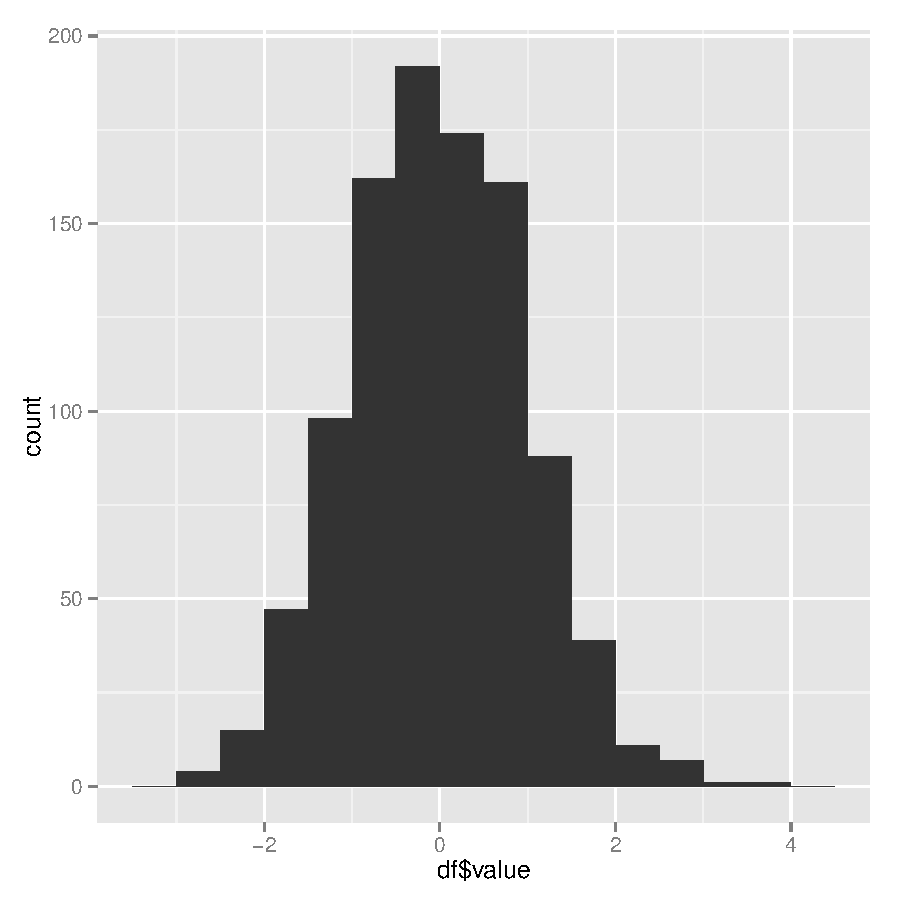
\includegraphics{cookbook-032}

More specifically, we can control the graphing using \textbf{geom\_histogram}

\begin{Schunk}
\begin{Sinput}
> ggplot(df, aes(x=value)) + geom_histogram(binwidth=.5, colour="black", fill="white")
\end{Sinput}
\end{Schunk}
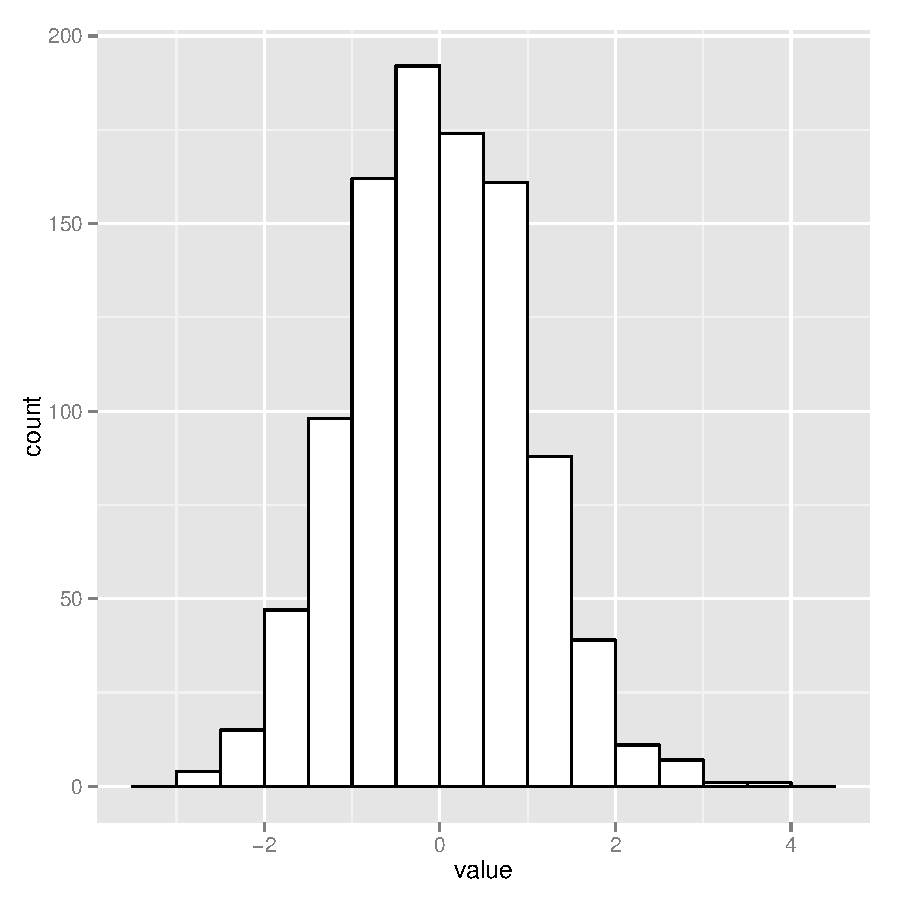
\includegraphics{cookbook-033}

To draw a probability density function (pdf) over the histogram

\begin{Schunk}
\begin{Sinput}
> ggplot(df, aes(x=value)) + 
+ geom_histogram(aes(y=..density..),
+                binwidth=.5,
+                colour="black", fill="white") +
+ geom_density(alpha=.2, fill="#FF6666") +
+ geom_vline(aes(xintercept=mean(value, na.rm=T)),
+            color="red", linetype="dashed", size=1)
\end{Sinput}
\end{Schunk}
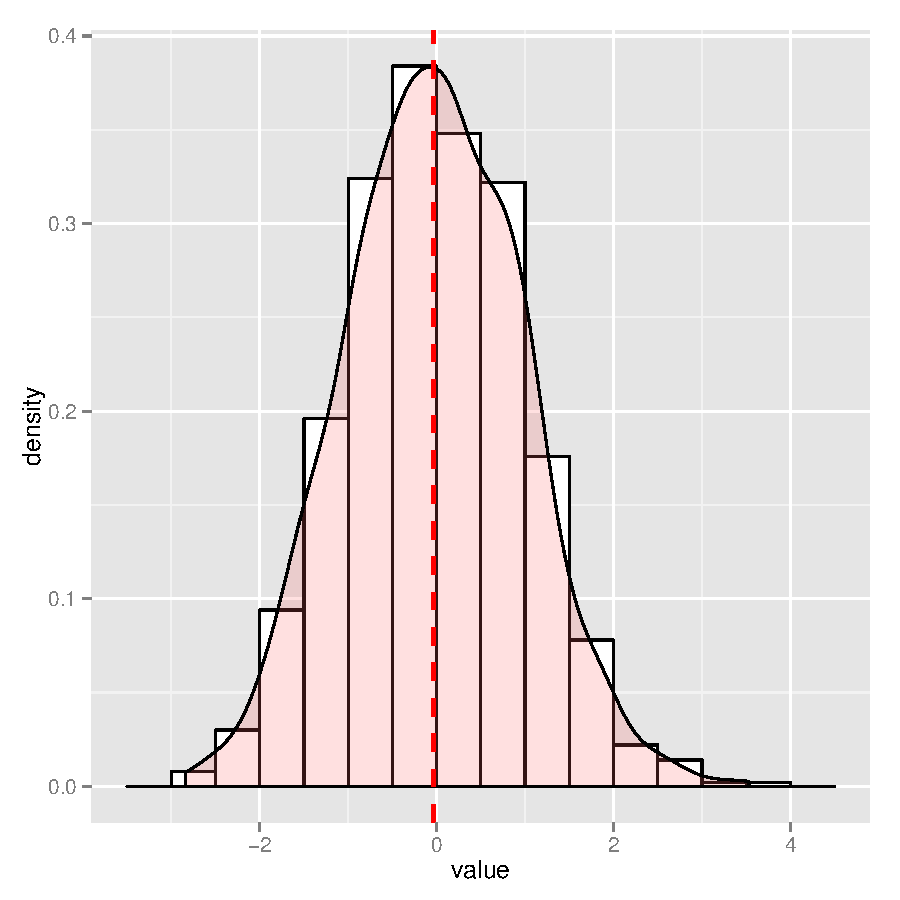
\includegraphics{cookbook-034}

\subsection{Line Graphs, Smoothing}

Say we have a time series and would like to plot it in ggplot.
We can plot it as a scatterplot, then draw a straight line through it
using a linear regression

\begin{Schunk}
\begin{Sinput}
> x = rnorm(100)
> y = 1 + 3*x + x^2
> df = data.frame(y = y, x = x)
> ggplot(df, aes(x=x,y=y)) + 
+ geom_point(shape=1) +
+ geom_smooth(method=lm, se=T)
\end{Sinput}
\end{Schunk}
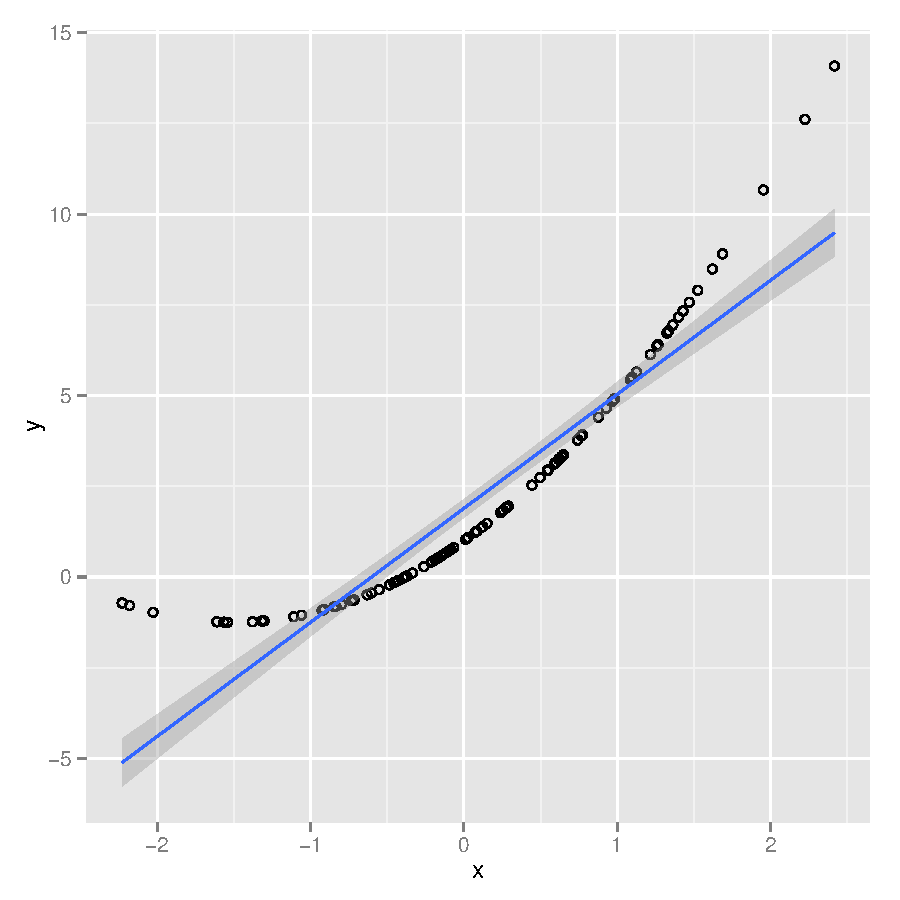
\includegraphics{cookbook-035}

Alternativley, we could use LOESS to fit the data points,
which fits a polynomial curve instead of a straight line.

\begin{Schunk}
\begin{Sinput}
> ggplot(df, aes(x=x,y=y)) + 
+ geom_point(shape=1) +
+ geom_smooth()
\end{Sinput}
\end{Schunk}
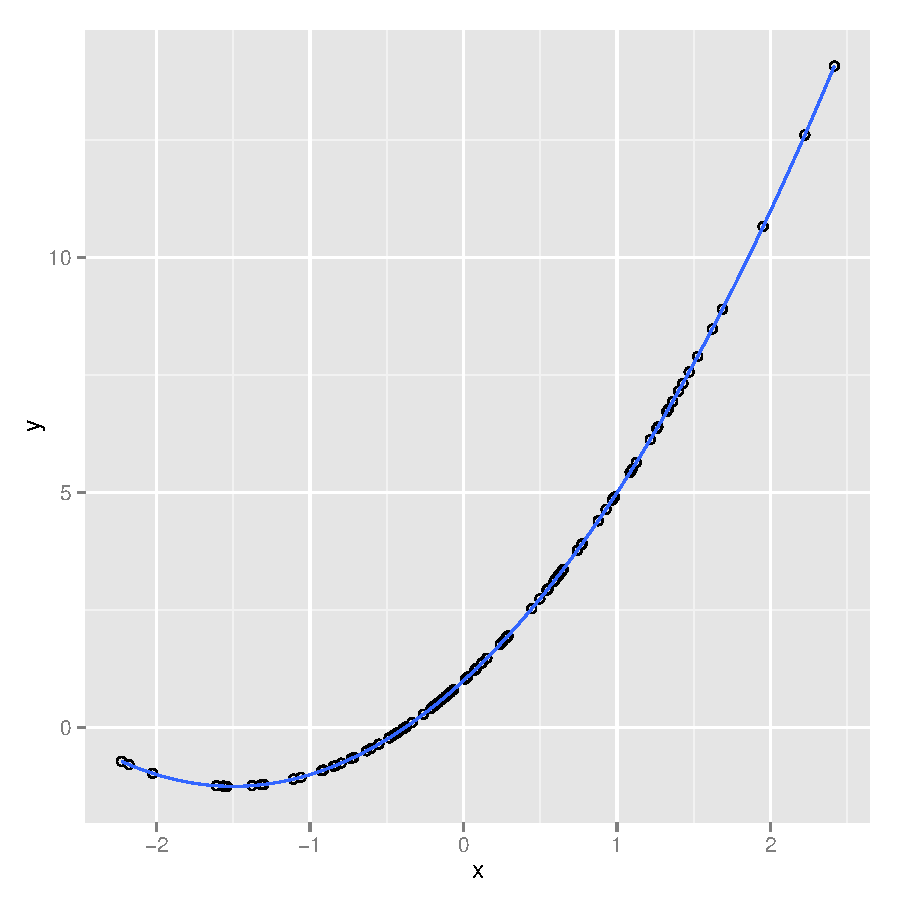
\includegraphics{cookbook-036}

\subsection{Faceting the Electric Load Data}

Faceting is a way to see partitions of data side by side.  Let's refer back
to the Kaggle Load Data.  Say we would like to do a comparison across the
weekdays Monday vs Tuesday vs Wednesday, etc.  ggplot likes working with 
data in the long format, so we will refer to the dataset \textit{data.long}
we created earlier.

\begin{Schunk}
\begin{Sinput}
> head(data.long)
\end{Sinput}
\begin{Soutput}
  zone_id year month day       date variable value
1       1 2004     1   1 2004-01-01       h1 16853
2       1 2004     1   2 2004-01-02       h1 14155
3       1 2004     1   3 2004-01-03       h1 14439
4       1 2004     1   4 2004-01-04       h1 11273
5       1 2004     1   5 2004-01-05       h1 10750
6       1 2004     1   6 2004-01-06       h1 15742
\end{Soutput}
\end{Schunk}

First, we need more data munging.  We know that date and variable together
form a datetime.  Again, let us create a proper datetime object.

\begin{Schunk}
\begin{Sinput}
> hour = as.numeric(str_extract(data.long$variable, "\\d+"))
> datetime = data.long$date + 60 * 60 * hour
> data.long$datetime = datetime
> head(data.long)
\end{Sinput}
\begin{Soutput}
  zone_id year month day       date variable value            datetime
1       1 2004     1   1 2004-01-01       h1 16853 2004-01-01 01:00:00
2       1 2004     1   2 2004-01-02       h1 14155 2004-01-02 01:00:00
3       1 2004     1   3 2004-01-03       h1 14439 2004-01-03 01:00:00
4       1 2004     1   4 2004-01-04       h1 11273 2004-01-04 01:00:00
5       1 2004     1   5 2004-01-05       h1 10750 2004-01-05 01:00:00
6       1 2004     1   6 2004-01-06       h1 15742 2004-01-06 01:00:00
\end{Soutput}
\begin{Sinput}
> str(data.long)
\end{Sinput}
\begin{Soutput}
'data.frame':	792000 obs. of  8 variables:
 $ zone_id : int  1 1 1 1 1 1 1 1 1 1 ...
 $ year    : int  2004 2004 2004 2004 2004 2004 2004 2004 2004 2004 ...
 $ month   : int  1 1 1 1 1 1 1 1 1 1 ...
 $ day     : int  1 2 3 4 5 6 7 8 9 10 ...
 $ date    : POSIXct, format: "2004-01-01" "2004-01-02" ...
 $ variable: Factor w/ 24 levels "h1","h2","h3",..: 1 1 1 1 1 1 1 1 1 1 ...
 $ value   : num  16853 14155 14439 11273 10750 ...
 $ datetime: POSIXct, format: "2004-01-01 01:00:00" "2004-01-02 01:00:00" ...
\end{Soutput}
\end{Schunk}

One thing we should make sure is that zone\_id is recognized as a categorical
variable.  While it takes on values that are pure numbers, it will be helpful
for us to define it as a categorical variable so we can take advantage of groups
in our plots

\begin{Schunk}
\begin{Sinput}
> data.long$zone_id = as.factor(data.long$zone_id)
> head(data.long)
\end{Sinput}
\begin{Soutput}
  zone_id year month day       date variable value            datetime
1       1 2004     1   1 2004-01-01       h1 16853 2004-01-01 01:00:00
2       1 2004     1   2 2004-01-02       h1 14155 2004-01-02 01:00:00
3       1 2004     1   3 2004-01-03       h1 14439 2004-01-03 01:00:00
4       1 2004     1   4 2004-01-04       h1 11273 2004-01-04 01:00:00
5       1 2004     1   5 2004-01-05       h1 10750 2004-01-05 01:00:00
6       1 2004     1   6 2004-01-06       h1 15742 2004-01-06 01:00:00
\end{Soutput}
\begin{Sinput}
> str(data.long)
\end{Sinput}
\begin{Soutput}
'data.frame':	792000 obs. of  8 variables:
 $ zone_id : Factor w/ 20 levels "1","2","3","4",..: 1 1 1 1 1 1 1 1 1 1 ...
 $ year    : int  2004 2004 2004 2004 2004 2004 2004 2004 2004 2004 ...
 $ month   : int  1 1 1 1 1 1 1 1 1 1 ...
 $ day     : int  1 2 3 4 5 6 7 8 9 10 ...
 $ date    : POSIXct, format: "2004-01-01" "2004-01-02" ...
 $ variable: Factor w/ 24 levels "h1","h2","h3",..: 1 1 1 1 1 1 1 1 1 1 ...
 $ value   : num  16853 14155 14439 11273 10750 ...
 $ datetime: POSIXct, format: "2004-01-01 01:00:00" "2004-01-02 01:00:00" ...
\end{Soutput}
\end{Schunk}

One way to see many partitions of a dataset in a graph is to group the
data points and color them according to their partitions.  Alternatively, we
could also generate multiple graphs and put them side by side, faceting them.
For this example we will plot both.

First, we define the aes by plotting datetime on the x-axis, and value on the
y-axis.  The color of the lines will be determined by zone\_id

\begin{Schunk}
\begin{Sinput}
> ggplot(data.long, aes(x = datetime, y = value, color = zone_id)) +
+ geom_line()
\end{Sinput}
\end{Schunk}
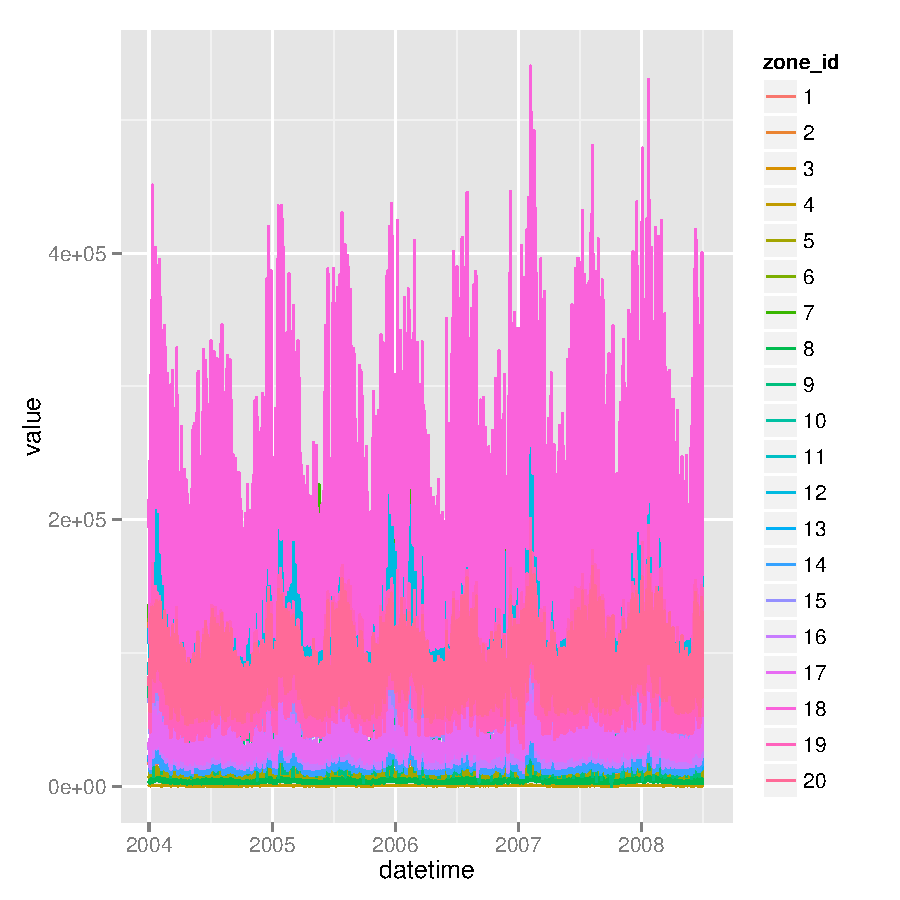
\includegraphics{cookbook-040}

To split this one graph into a grid of smaller graphs for side by side
comparison, we add facet\_wrap.  We will facet on zone\_id so that each
zone has a separate graph.

\begin{Schunk}
\begin{Sinput}
> ggplot(data.long, aes(x = datetime, y = value, color = zone_id)) +
+ geom_line() + facet_wrap(~zone_id, ncol = 5)
\end{Sinput}
\end{Schunk}
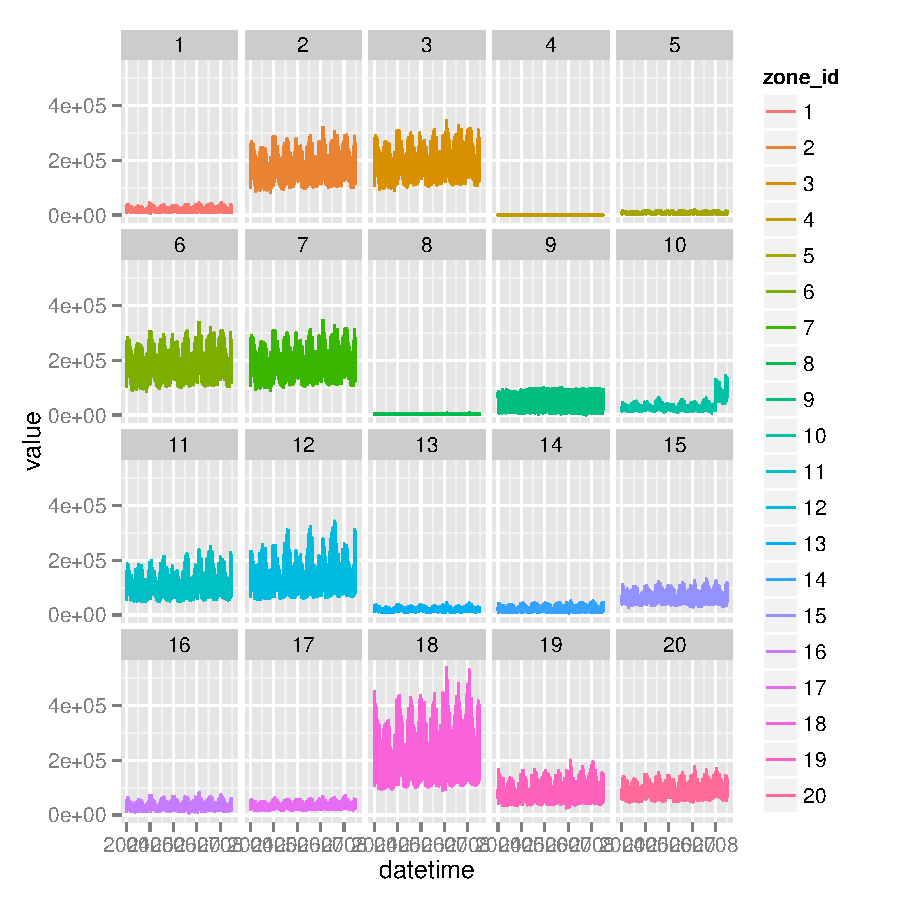
\includegraphics{cookbook-041}

These graphs don't tell us much because the line graphs have too many points.
Instead, we could take a subset of this data by looking at the time period
January 2004 only

\begin{Schunk}
\begin{Sinput}
> ggplot(subset(data.long, (year == 2004 & month == 1)),
+        aes(x = datetime, y = value, color = zone_id)) +
+ geom_line() + facet_wrap(~zone_id, ncol = 5)
\end{Sinput}
\end{Schunk}
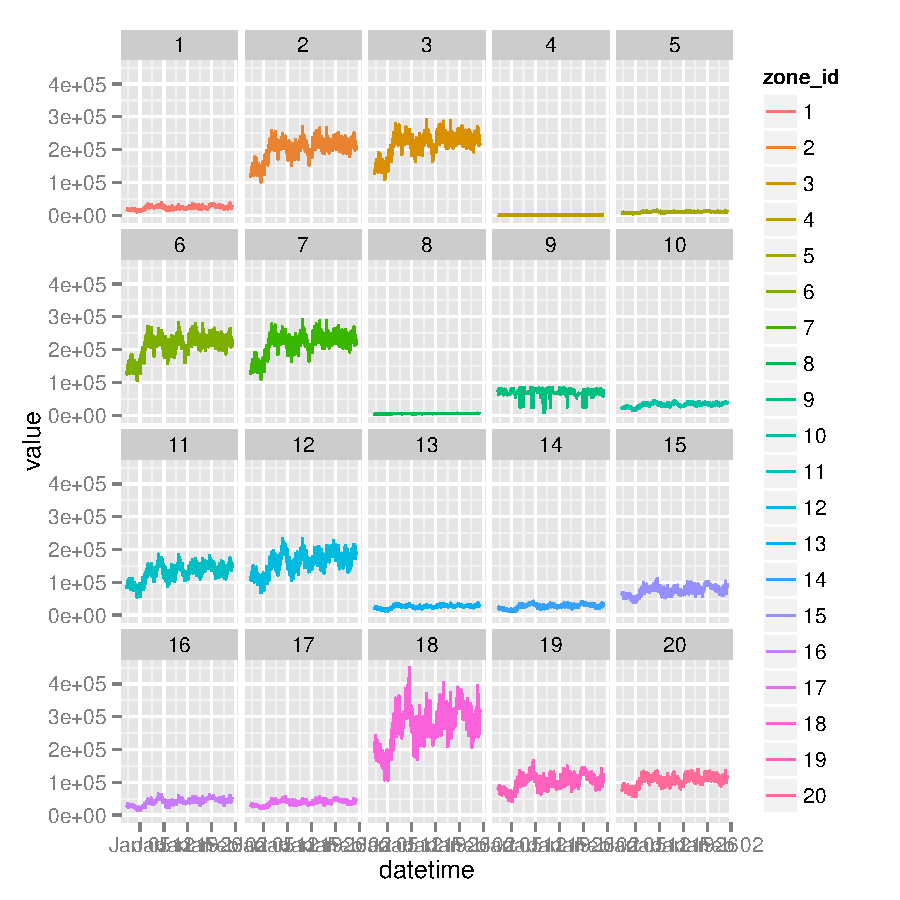
\includegraphics{cookbook-042}

\section{Data Modeling}

Models are mathematical constructs that are used to explain data.  What
does it mean to ``explain'' data?  In social sciences where statistics is most
often used, data is never consistent.  It always has variation, whether
systematic variation caused by changes in a controlled environment or by unknown
randomness.  Models try to identify these variations, and explain why they happen.
Within this field of models there are two strong schools of thought: 
\textbf{predictive models} and parsimonious, \textbf{data models}.

Predictive models do their utmost best to predict new data points.  These models
identify variation, but they do not necessarily come up with intuitive
ways to explain the variation.  A predictive model can be incredibly complex,
but will still be popular if it makes good predictions.  This school of thought
is popular in machine learning.

Data models will not be as good in prediction as predictive models, but they
aim to be better at explaining variance.  These models are designed to be simple
and parsimonious.  They utilize only a few variables and the model formula
has a simple form.  Usually data models are appropriate when we need to make
\textbf{inferences}, that is we need to understand to what degree each variable
impacts the outcome, which variables are significant, what the covariances are...

\subsection{Regression}

Performing a linear regression is done with the lm command.  Say we have
data that, unknown to us, is generated using the formula $y = 1 + 3x + x^2$
If we wanted to fit a linear model to data points x and y, we could come
up with the fit

\begin{Schunk}
\begin{Sinput}
> x = rnorm(100)
> y = 1 + 3*x + x^2 + rnorm(100)
> y.lm = lm(y ~ x)
> summary(y.lm)
\end{Sinput}
\begin{Soutput}
Call:
lm(formula = y ~ x)

Residuals:
    Min      1Q  Median      3Q     Max 
-2.9056 -1.2193 -0.3100  0.8329  7.8503 

Coefficients:
            Estimate Std. Error t value Pr(>|t|)    
(Intercept)   2.0811     0.1845   11.28   <2e-16 ***
x             2.5973     0.1726   15.05   <2e-16 ***
---
Signif. codes:  0 ‘***’ 0.001 ‘**’ 0.01 ‘*’ 0.05 ‘.’ 0.1 ‘ ’ 1 

Residual standard error: 1.844 on 98 degrees of freedom
Multiple R-squared: 0.698,	Adjusted R-squared: 0.6949 
F-statistic: 226.5 on 1 and 98 DF,  p-value: < 2.2e-16 
\end{Soutput}
\end{Schunk}

\subsection{Generalized Linear Models}

\subsection{Neural Networks}

\subsection{CART: Classification and Regression Tree}

\section{Advanced Data Analysis}

\subsection{Penalized Models}

\subsection{Boosting}

\section{Open Source Development}

\subsection{devtools}

\subsection{Roxygen}

\subsection{Non-R Source Code}

\end{document}
